\documentclass[runningheads]{llncs}
\usepackage[T1]{fontenc}
\usepackage[utf8]{inputenc}
\usepackage{graphicx}
\usepackage{booktabs}
\usepackage{array}
\usepackage{url}
\graphicspath{{../figures/phase2/}}
\begin{document}
\title{NashForge: One Instrument for Three Learning Families in Heads-Up No-Limit Hold'em, and What a Live Arena Adds}
\titlerunning{NashForge: one instrument for three learning families}
\author{Dheirav Prakash}
\authorrunning{D. Prakash}
\institute{Department of Computer Science and Engineering, College of Engineering Guindy, Anna University, Chennai, India \\ \email{dheirav2005@gmail.com}}
\maketitle
\begin{abstract}
Heads-up no-limit Texas hold'em is the standard testbed for decision making under imperfect information, and three families of method claim it: regret-minimisation solvers, evolutionary search over policies, and deep reinforcement learning. They are rarely compared on one instrument. NashForge builds that instrument: one engine, one card and betting abstraction, and one evaluation protocol (40,000-hand matches against a fixed panel with standard errors), and trains all three families against it. The solver, external-sampling Monte Carlo CFR with its core rewritten in C++ (32.5 times faster, a 250,000-iteration strategy in 109 s), beats the evolutionary agent by 212 BB/100 and the PPO agent by 75 BB/100, and neither learned family closes the gap with more training. Two abstraction results follow from the same instrument: six hand-strength buckets beat twenty at every training budget, and the reason is the equity estimator's noise, which misplaces 42 percent of hands at 40 samples; at 200 samples the solver improves by +5.9 $\pm$ 1.9 BB/100. Phase 2 adds what no fixed panel can give: the solver deployed as a rated bot on a public arena against other developers' bots, with every decision logged. 73 matches and 2,850 hands located the abstraction's weakest point in our own data, deep-stacked re-raised pots, and four fixes were built and measured against it in one day. We report the metrics, the diagnosis and the fixes.
\end{abstract}
\keywords{counterfactual regret minimization \and imperfect-information games \and abstraction \and evolutionary search \and proximal policy optimization \and poker \and evaluation}
\section{Introduction and Problem Statement}
A poker bot is a strategy for a game the player cannot see all of. The state of the art solves an abstraction of the game with counterfactual regret minimisation (CFR) and its Monte Carlo variants [2, 3], and the same abstraction question, how coarsely a game can be represented and still be played well, decides everything downstream [6, 7]. Two other families claim the same problem: evolutionary search over policy parameters [17] and deep reinforcement learning by self-play [14, 15]. Published comparisons between the three are rare and usually indirect, because each family is measured on its own instrument.

The problem this project set itself is therefore an instrument, not a bot: one engine whose rules and chip accounting are audited, one abstraction shared by every agent, and one evaluation protocol with error bars, so that a claim like ``the solver beats PPO by 75 BB/100'' means what it says. Phase 1 built the instrument and validated the solver on games with known answers. Phase 2, reported here, produced the comparison, two abstraction findings, a native core that made the solver fast enough to experiment with, and a deployment against live opponents that found the abstraction's weakest point and fixed it.

Two constraints shaped the work and are worth stating. Every result in this paper carries a standard error and the number of hands it was measured over, because an earlier version of the project published a comparison against an under-trained solver and had to withdraw it; the instrument's own history is the strongest argument for the instrument. And nothing is quoted from a partial run: a favourable-looking partial is the exact shape of the stopping-rule error that invalidates sequential tests.

\section{Literature Survey and the Gap}
Regret minimisation. Zinkevich et al. [2] introduced CFR, which minimises counterfactual regret at every information set and whose average strategy converges to a Nash equilibrium in two-player zero-sum games. Lanctot et al. [3] made it practical for large games with Monte Carlo sampling; the external-sampling variant used here samples the opponent's and chance's actions and walks every action of the player being updated. CFR+ [4] and discounted CFR [5] accelerate convergence in the full-traversal setting; under sampling we measured both as worse than linear weighting on Leduc, which is why the solver uses linear CFR.

Abstraction. Johanson et al. [6] evaluate state-space abstractions by the exploitability of the strategies they produce and show that finer is not always better; Waugh et al. [7] give the pathologies that a refined abstraction can introduce. Ganzfried and Sandholm [8] address the other side, the action abstraction, with translation: a bet size outside the abstraction is mapped probabilistically onto its neighbours rather than rounded, because a deterministic boundary is a thing an opponent sits just inside of. This project's bridge to live opponents is their pseudo-harmonic mapping.

The superhuman systems. DeepStack [11], Libratus [12] and Pluribus [13] combine CFR-family solving with real-time search and, in Libratus, an unbounded action tree during play. Lisý and Bowling [10] measured how far short of equilibrium the strong public bots fall with a local best response, and Slumbot, the standard free benchmark, remains the reference point for a solver built on a laptop.

The other families. Proximal policy optimisation [14] and neural fictitious self-play [15] apply deep reinforcement learning to imperfect-information games; Deep CFR [16] replaces tabular regrets with networks. Evolution strategies [17] are the population-based alternative, and Bayes' Bluff [9] is the classic treatment of the opponent-modelling problem that equilibrium play sets aside.

The gap. Each of these families is evaluated on its own terms: exploitability for solvers, reward curves for reinforcement learning, fitness for evolution. A reward curve at 3,000 hands has an error bar of $\pm$57 BB/100, which this project measured and then spent a phase learning not to read. What the literature lacks, and what a course project can supply, is one instrument that puts all three families in the same game with the same abstraction and the same error bars, and then a check of that instrument against opponents that were not built by us. The second half of that gap is the phase-2 contribution: live, rated play against other developers' bots, logged decision by decision, used to find where the abstraction fails.

\section{Methodology}
\subsection{Overall Architecture}
Figure 1 shows the system. The engine (rules, chips, hand evaluation) survived an audit unchanged and is the one part everything else is built on. The abstraction layer maps a hand to one of six strength classes per street by its equity against a random hand, optionally combined with the board's texture, and maps betting to six actions: fold, check or call, raises of half, one and two times the pot, and all-in. The three agent families share the abstraction and the engine and are evaluated by one protocol: 40,000-hand matches against a fixed panel of a uniform-random player, an always-call player and the converged solver, reported as big blinds per hundred hands with standard errors and the rate at which the solver's lookup missed. Two external instruments sit beside the panel: Slumbot, and the Chipzen arena, where the solver plays rated matches against other developers' bots.

\begin{figure}[t]
\centering
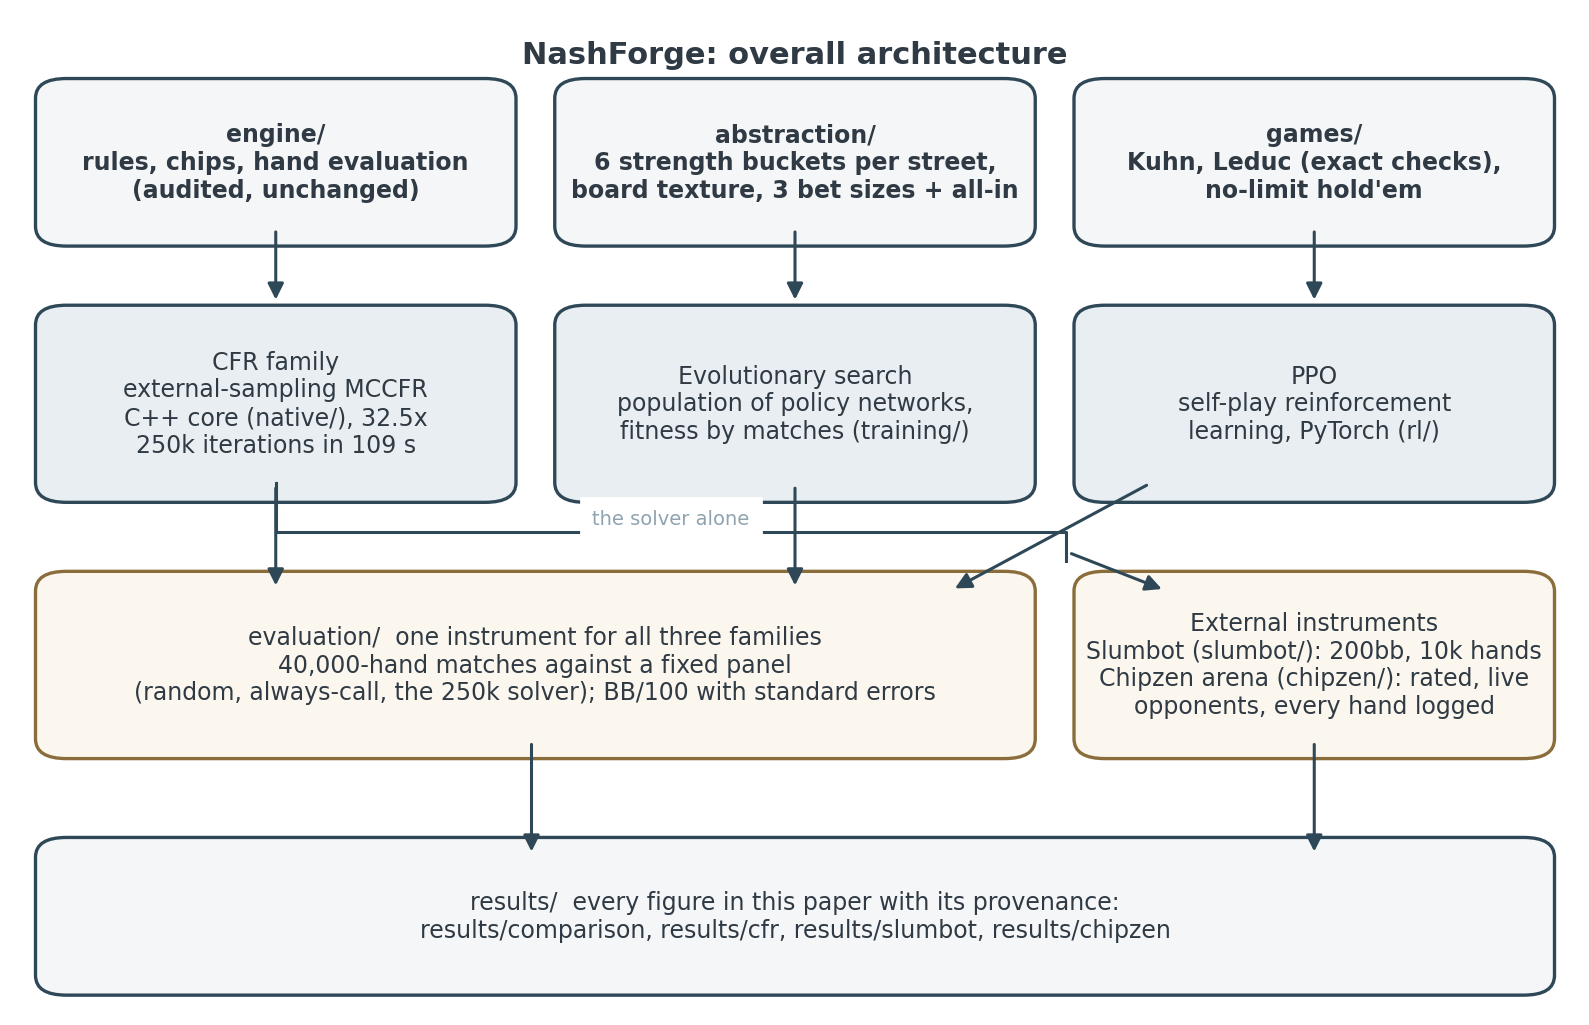
\includegraphics[width=12.2cm]{fig_architecture.png}
\caption{Overall architecture. The engine and abstraction are shared; the three families are measured on one internal instrument and the solver on two external ones.}
\label{fig:1}
\end{figure}

\subsection{Module: the Solver (CFR family)}
The solver is external-sampling MCCFR [3] with linear weighting over the abstracted game, keyed on the string bucket\textbar{}history, where bucket is the hand's class and history the sequence of abstract actions with a separator per street. It is validated on Kuhn poker, where it reproduces the analytic game value of $-$1/18 exactly, and on Leduc, where exploitability is computed exactly. The inner loop was ported to C++ (a nanobind extension of about 1,500 lines: hand evaluator, equity sampler, betting, MCCFR) and verified against the Python on every one of 6,216 enumerated betting sequences; the two produce the same distribution of buckets and play indistinguishably. The port made a 250,000-iteration solver a 109-second job instead of a 4.8-hour one, which is what made the experiments of Section 4 affordable.

\subsection{Module: Evolutionary Search}
A population of small policy networks over hand-crafted features, selected by tournament fitness measured in matches and bred with crossover and mutation. Fifty generations consumed 36,000,000 hands. The fitness signal's repeatability was measured at r = +0.12 at the real budget, which bounds what selection can do, and is reported rather than hidden.

\subsection{Module: Proximal Policy Optimisation}
A PyTorch actor-critic trained by self-play with PPO [14] over the same six actions, evaluated at 500,000, 2,000,000 and 8,000,000 hands of training. The checkpoints are produced by self-play only, never against the solver, so the comparison in Section 4 is between independently trained agents.

\subsection{Module: the Evaluation Instrument}
Every matchup is 40,000 hands with seats alternating, the same cards dealt to every agent in a panel, and the result reported as chips per hand with a standard error, converted to BB/100. The solver's lookup miss rate is reported with every figure, because a solver whose strategy has no entry for a situation is choosing at random there, and a measurement that did not report it once turned out to be a measurement of a random agent at a 74 percent miss rate.

\subsection{Module: the Arena Path (Phase 2)}
Figure 2 shows the deployment. The Chipzen platform sends a structured game state over a WebSocket at every decision; chipzen/client.py holds the lobby connection, reconnects, sits in the rated matchmaking queue, and logs every decision with the state it was taken from. chipzen/bridge.py turns the platform's action history into the solver's history key: each raise becomes a fraction of the pot after the call, translated onto the abstraction's sizes with the pseudo-harmonic mapping [8], with all-in judged against the bettor's real stack. chipzen/player.py holds a ladder of solvers, one per effective stack depth from 5 to 200 big blinds, because arena matches carry stacks over between hands and step the blinds up every twenty hands; a hand is answered by the rung nearest its depth in ratio. A node the main solver never stored (under one raise per street, any re-raise) is put first to a deeper-tree companion solver and only then to a hand-strength rule. chipzen/opponents.py counts, per opponent and across matches, how they answer our bets, and withholds bluffs from a bot that folds to fewer than a quarter of them over at least a hundred.

\begin{figure}[t]
\centering
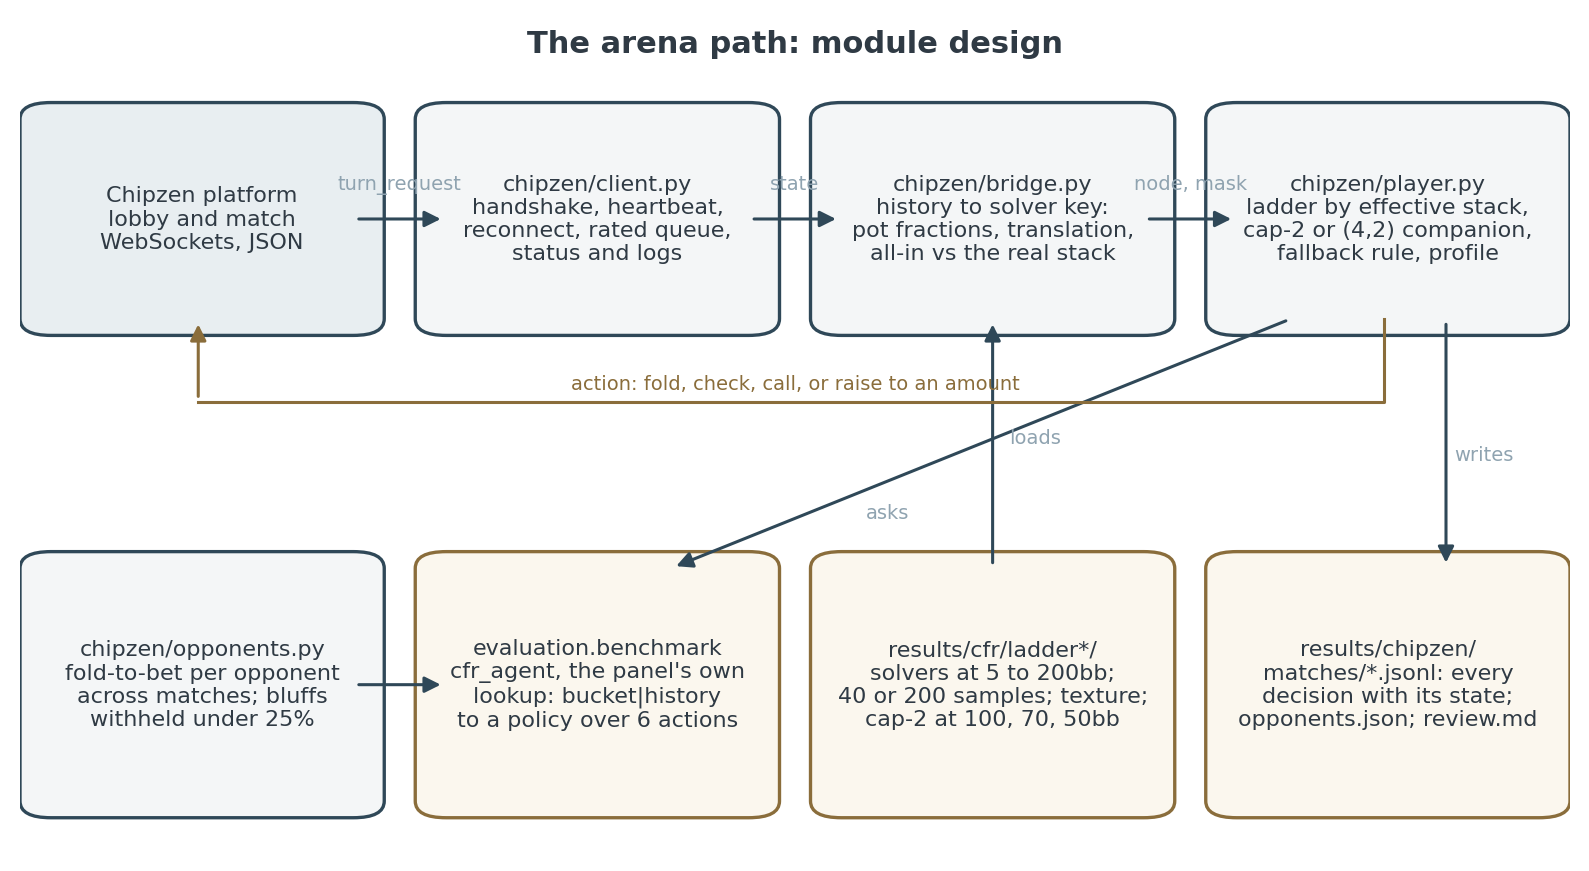
\includegraphics[width=12.2cm]{fig_arena_modules.png}
\caption{Module design of the arena path. The lookup is the panel's own cfr\_agent, so the rating is earned by the agent that was measured.}
\label{fig:2}
\end{figure}

\section{Results and Analysis}
\subsection{Validation on Solved Games}
On Kuhn poker the solver's average strategy reaches the analytic value of $-$1/18 for the first player; the C++ core reproduces it exactly. On Leduc, exact exploitability falls monotonically with iterations and linear CFR was 10 percent better than vanilla at equal iterations, while CFR+ and discounted CFR were worse under sampling. These are the checks that make the no-limit results readable.

\subsection{Three Families on One Panel}
Table 1 and Fig. 3 give the phase-4 comparison: every row measured on the same panel, 40,000 hands per matchup, against a solver trained by the C++ core. Both learned families lose to the solver, PPO by about 75 BB/100 at every training rung and evolution by 212. More training does not close PPO's gap: the three rungs are $-$84.6, $-$72.5 and $-$74.9, flat within their intervals. Evolutionary search spent seventy-two times as many hands as PPO's smallest rung and finished 127 BB/100 further behind; that comparison survived a change of panel and a change of solver implementation, and is the firm result. Fifty generations of evolution were nonetheless worth +43.9 $\pm$ 20 BB/100 over the untrained population against the solver: a noisy ranking signal and a real improvement are compatible.

\begin{table}[t]
\caption{The comparison, BB/100 to the row agent, 40,000 hands per matchup (results/comparison/phase4\_native.json).}
\label{tab:1}
\centering
\small
\begin{tabular}{lrrrr}
\toprule
agent & training hands & vs random & vs always-call & vs CFR solver \\
\midrule
CFR solver, 250k iterations & self-play & +258.7 & +647.3 & — \\
Evolution, 50 generations & 36,000,000 & +202.7 & -0.2 & -211.8 \\
PPO & 500,000 & +191.2 & +372.6 & $-$84.6 \\
PPO & 2,000,000 & +137.2 & +373.2 & $-$72.5 \\
PPO & 8,000,000 & +226.8 & +329.1 & $-$74.9 \\
\bottomrule
\end{tabular}
\end{table}

\begin{figure}[t]
\centering
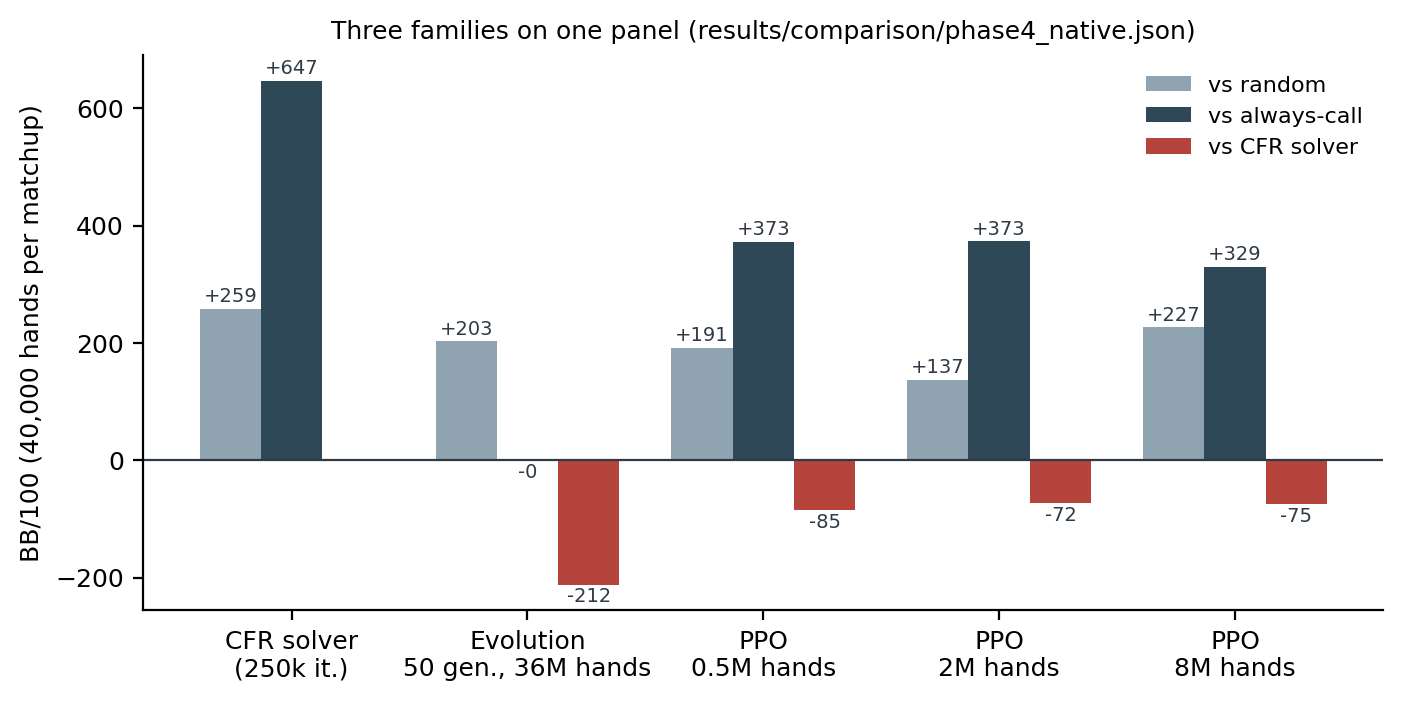
\includegraphics[width=12.2cm]{fig_panel.png}
\caption{The three families against the panel. The baselines cannot rank agents: a less converged solver beats always-call by more, so only the solver column separates them.}
\label{fig:3}
\end{figure}

An instrument lesson came with this table. An earlier panel used a 4,000-iteration solver, about two minutes of training, against which PPO appeared to win by +36 BB/100 and evolution appeared to have learned nothing. Both readings were correct measurements against an opponent too weak to distinguish anything, and the errors point in opposite directions because an under-trained solver is far more exploitative than a converged one. Changing the instrument overturned the finding; new data did not. Every figure here is from the converged panel.

\subsection{The Card Abstraction}
Six strength buckets against twenty, trained at equal wall-clock budgets over a 128-fold range and played head to head (Fig. 4): six wins at every budget, and the gap plateaus around +0.5 chips per hand rather than crossing. Twenty was not short of compute; it bought more iterations per second and still lost. The reason is the estimator. Equity is estimated by 40 Monte Carlo rollouts, whose standard deviation of 0.067 is about half the spacing between adjacent bucket centroids (0.10 to 0.17), so 42 percent of hands change bucket when re-rolled. The sweep measured how many buckets the estimator can resolve, not how many are worth having. Raising the sample count to 200 (standard deviation 0.031) produced a solver that beats the 40-sample one by +5.9 $\pm$ 1.9 BB/100 over three seeds of 40,000 hands, on the same betting tree (Fig. 5). The precision was affordable only after the port.

\begin{figure}[t]
\centering
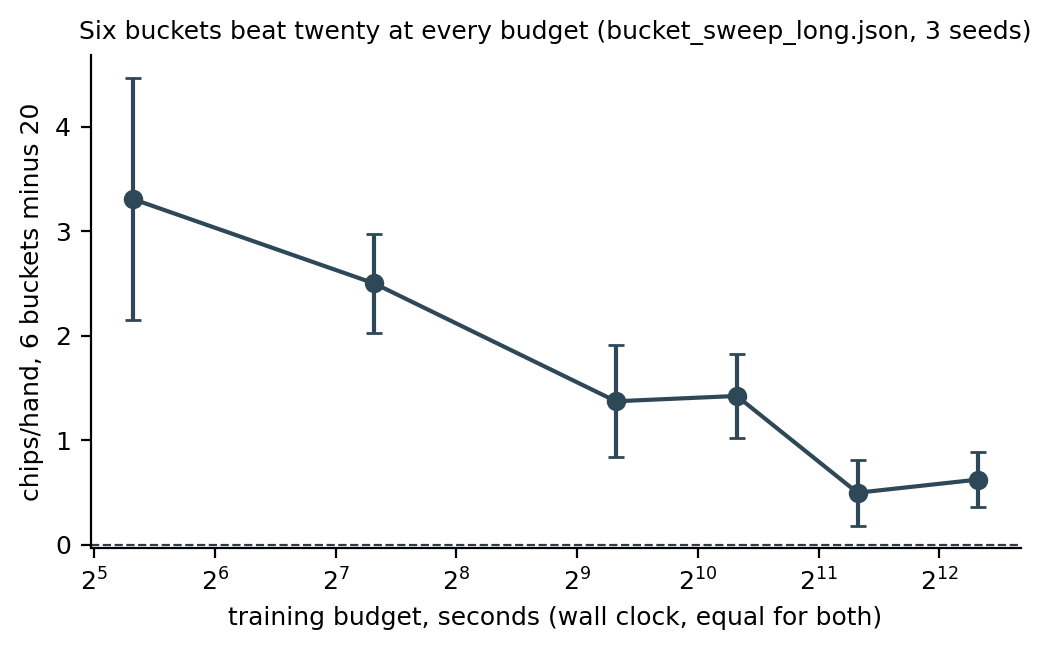
\includegraphics[width=10.5cm]{fig_bucket_sweep.png}
\caption{Six buckets minus twenty, chips per hand, at equal wall-clock training budgets; 95 percent intervals across three seeds.}
\label{fig:4}
\end{figure}

\begin{figure}[t]
\centering
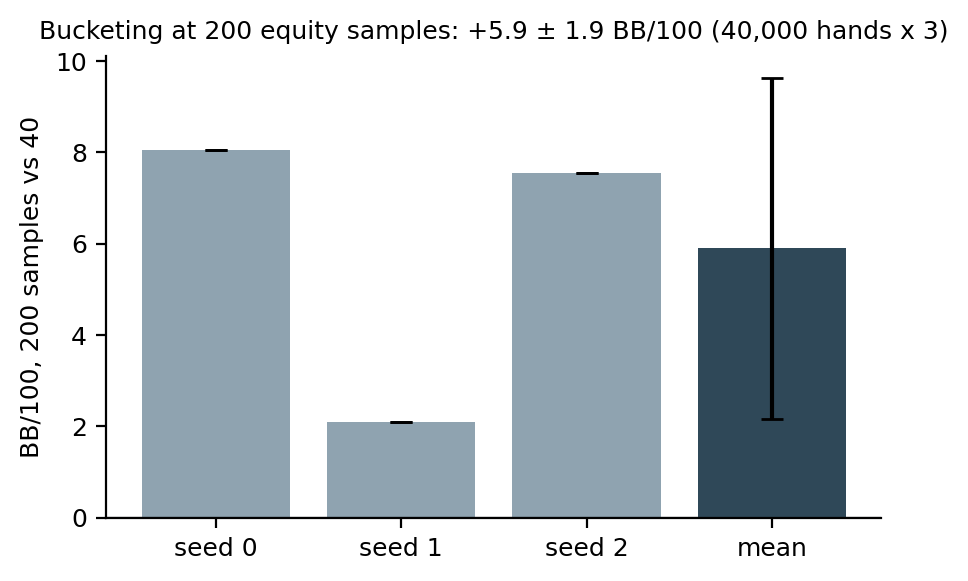
\includegraphics[width=9.5cm]{fig_eq200.png}
\caption{The 200-sample estimator against the 40-sample one, same tree, three seeds of 40,000 hands.}
\label{fig:5}
\end{figure}

\subsection{Speed}
Fig. 6 gives the solver's per-iteration cost across the phase: 32.4 ms in Python, 7.47 ms after compiling the hand evaluator and moving the rollout's sampling inside it, and 0.44 ms in the C++ core, a 32.5-fold end-to-end gain that turned a 4.8-hour solver into a 109-second one. Seven other optimisations were tried and reverted as neutral or worse, including suit isomorphism on the runtime cache; a profiler's per-call overhead had ranked them wrongly, which is recorded so they are not tried again.

\begin{figure}[t]
\centering
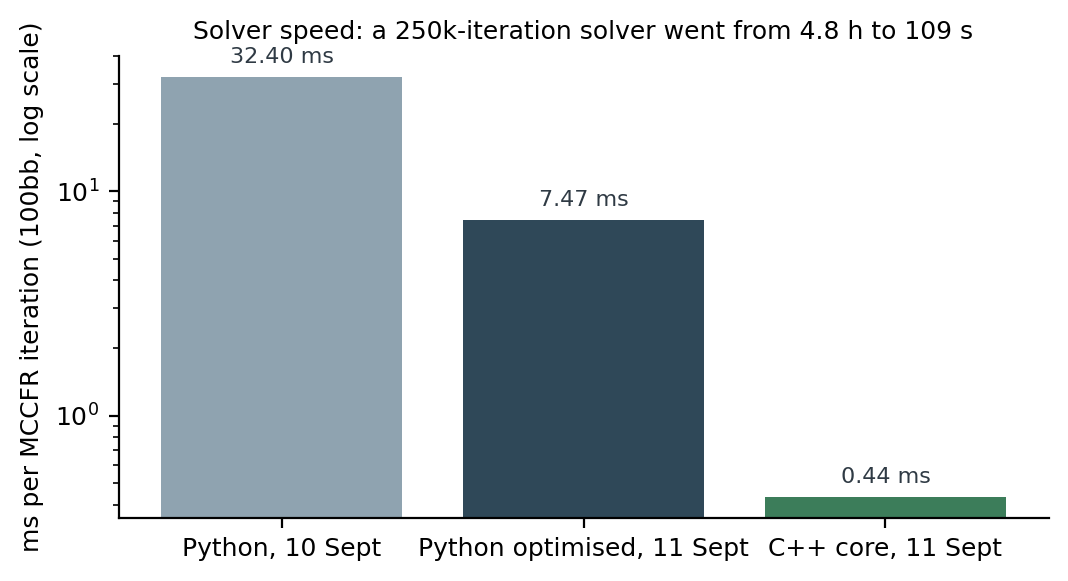
\includegraphics[width=10.0cm]{fig_speed.png}
\caption{Milliseconds per MCCFR iteration at 100 big blinds, log scale.}
\label{fig:6}
\end{figure}

\subsection{Slumbot}
Against Slumbot over 9,999 hands each (Fig. 7): $-$1,750 $\pm$ 524 mbb/hand for the 4,000-iteration solver, $-$987 $\pm$ 374 at 150,000 iterations, and $-$998 $\pm$ 396 for a 250,000-iteration solver retrained at Slumbot's 200-big-blind depth. Training halved the gap; matching the depth did not move it, and the lookup miss rate rose from 8.7 to 11.9 percent as deeper stacks reached more nodes the one-raise abstraction cannot express. The training and depth levers are spent; the binding constraint is the betting abstraction, one raise per street and three sizes against an opponent with eleven sizes and unlimited raises.

\begin{figure}[t]
\centering
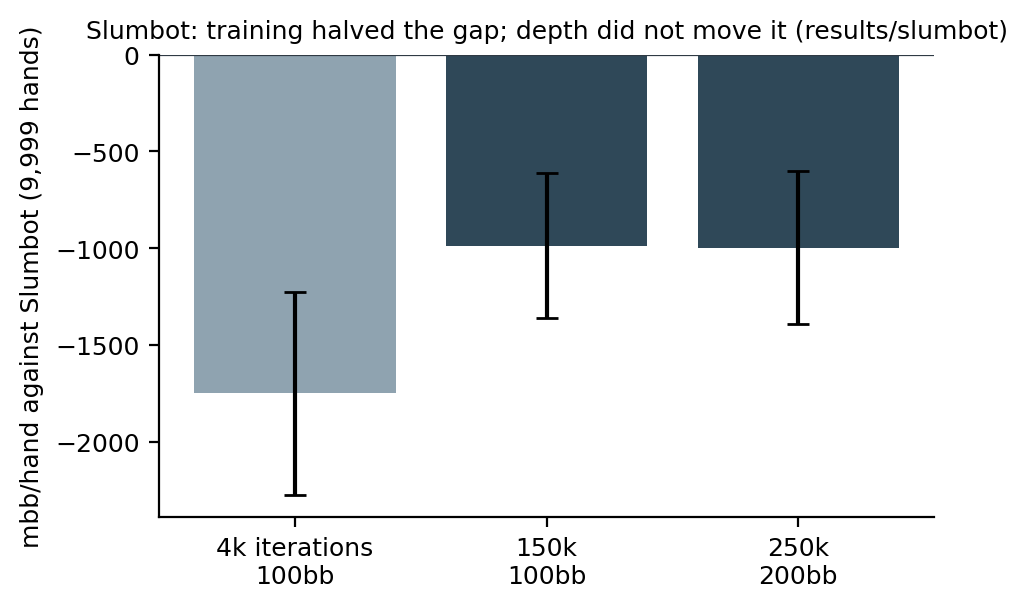
\includegraphics[width=9.5cm]{fig_slumbot.png}
\caption{Against Slumbot, milli-big-blinds per hand with 95 percent intervals, 9,999 hands each.}
\label{fig:7}
\end{figure}

\subsection{The Arena: Live, Rated Play}
On 13 September the solver was entered on the Chipzen arena as a remote bot: heads-up no-limit, 10,000 chips at blinds of 50 and 100, blinds stepping up every twenty hands, stacks carried over, matches played to a bust and rated by Glicko-2. Table 2 summarises every match logged to date: 73 matches (70 rated), 46 won, 2,850 hands, net +168,721 chips. Of 5,783 decisions, 356 (6 percent) had no entry in the one-raise solver; the companion answered 296 of them and the rule 60. No action was ever rejected by the platform, and the slowest decision took 142.7 ms against a 30-second clock. Showdowns: 329 won, 222 lost.

\begin{table}[t]
\caption{Arena matches by opponent (results/chipzen/matches, via scripts/chipzen\_review.py).}
\label{tab:2}
\centering
\small
\begin{tabular}{lrrrr}
\toprule
opponent & matches & won & hands & net chips \\
\midrule
hoops & 26 & 14 & 759 & +6,379 \\
r0ckGarden & 26 & 22 & 1538 & +172,342 \\
mr\_hide & 18 & 7 & 510 & -40,000 \\
PluriBot & 2 & 2 & 15 & +20,000 \\
pebble & 1 & 1 & 28 & +10,000 \\
\bottomrule
\end{tabular}
\end{table}

\begin{figure}[t]
\centering
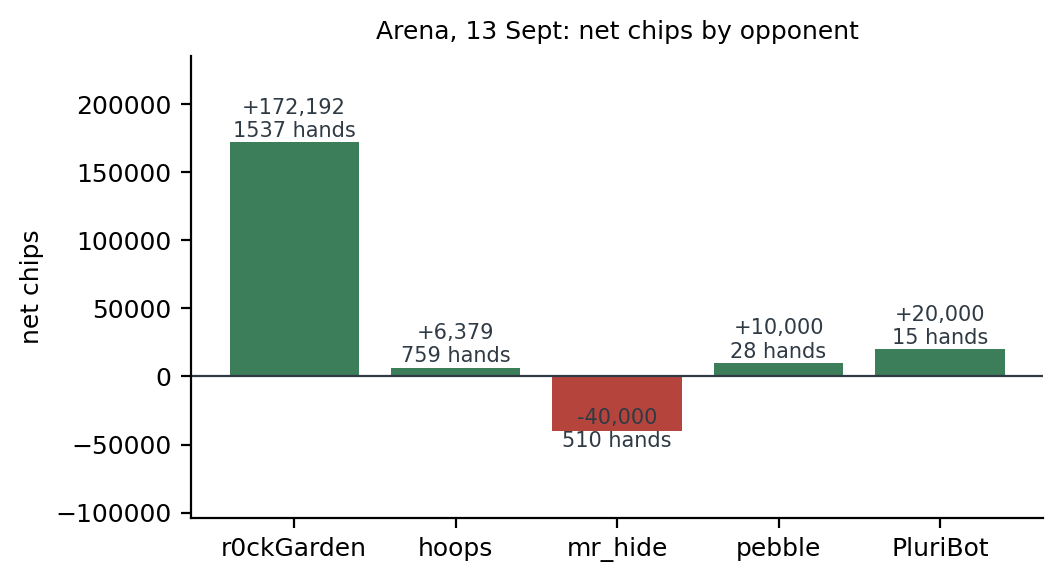
\includegraphics[width=10.0cm]{fig_arena_opponents.png}
\caption{Net chips by opponent. The bot crushes the weak bot, breaks even with the middle one, and loses to the one that re-raises.}
\label{fig:8}
\end{figure}

\subsection{Where the Chips Went, and Four Fixes}
Two cuts of the same data say the same thing (Fig. 9). By the effective stack at the start of the hand: -25,391 chips over 825 hands at 70 big blinds and deeper, against +144,723 over the 1422 hands below it. And by mechanism: in 12 hands the deeper-tree companion went all-in, 9 of them lost, net -53,608. The deep-stack game, where re-raised pots happen, is where the bot bleeds, and the reason is the same one Slumbot exposed: the main solver's tree has no re-raise, so every three-bet is answered by a substitute, and the substitute's only raise sizes were two pots and all-in. The second mechanism is the card abstraction reading hands without reading boards: two pair on a four-flush board sits in a good bucket and calls a bet that, from the range that bets there, is a flush.

Four fixes were built and tested the same evening. First, a companion shove with anything below the top strength class is taken as a call. Second, a full-size raise-cap-2 solver (every size on the re-raise, 390,456 information sets, 3,000,000 iterations, 2 h 12 min native) plays as the main solver at deep stacks; it exploits a calling station a third as hard as the one-raise solver (+204 against +647 BB/100), which is the price of knowing what a re-raise means. Third, the postflop bucket can carry the board's texture, six classes of flush and straight danger, mirrored in the C++ core and pinned equal on 3,000 random boards. Fourth, the opponent profile withholds bluffs from a bot whose fold-to-bet rate over a hundred bets is under a quarter; the bot that beat us folds to 14 percent. The season's rated rounds on the new solver set, against the matches above on the old one, are the before-and-after measurement.

\begin{figure}[t]
\centering
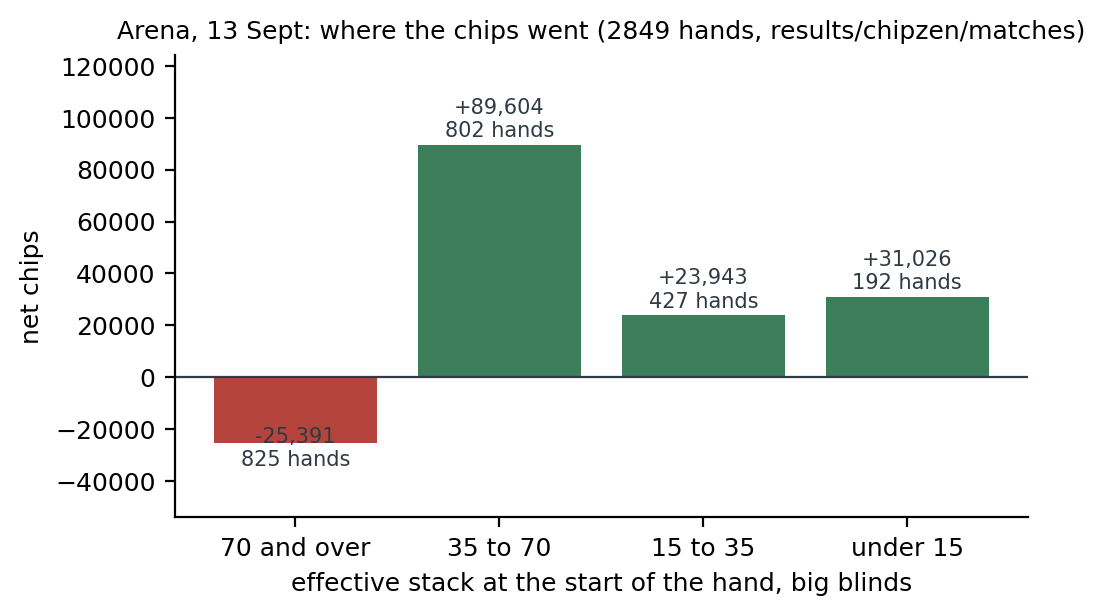
\includegraphics[width=10.0cm]{fig_arena_depth.png}
\caption{Net chips by effective stack depth at the start of the hand. Deep stacks are the re-raise game; shallow stacks are where the ladder wins.}
\label{fig:9}
\end{figure}

\section{Performance Metrics}
Table 3 lists every metric the project reports, what it measures, and the value at submission. Each is a number with an error bar or a count, never a curve read by eye.

\begin{table}[t]
\caption{Performance metrics and their values at submission.}
\label{tab:3}
\centering
\small
\begin{tabular}{lrr}
\toprule
metric & what it measures & value \\
\midrule
BB/100 with standard error & internal strength, 40,000 hands per matchup & solver over PPO +75, over evolution +212 \\
chips per hand, head to head & one abstraction against another, same budget & 6 buckets over 20: +0.62 $\pm$ 0.26 at 5,120 s \\
mbb/hand against Slumbot & distance from a strong external equilibrium & $-$998 $\pm$ 396 at 200bb \\
lookup miss rate & how often the strategy had no entry & 0.0\% on the panel; 11.9\% vs Slumbot; 6\% in the arena \\
ms per MCCFR iteration & training throughput & 32.4 (Python) to 0.44 (C++) \\
decision latency & play-time cost against the clock & 142.7 ms slowest, 30 s clock \\
arena record & rated play against other developers' bots & 46 of 73 matches, +168,721 chips \\
equity estimator sd & card abstraction precision & 0.067 at 40 samples, 0.031 at 200 \\
\bottomrule
\end{tabular}
\end{table}

Intermediate snapshots. Figs. 10 to 12 show the system at work rather than its outputs: the progress reader during a session, one logged hand as the review script prints it, and the training log of the raise-cap-2 solver.

\begin{figure}[t]
\centering
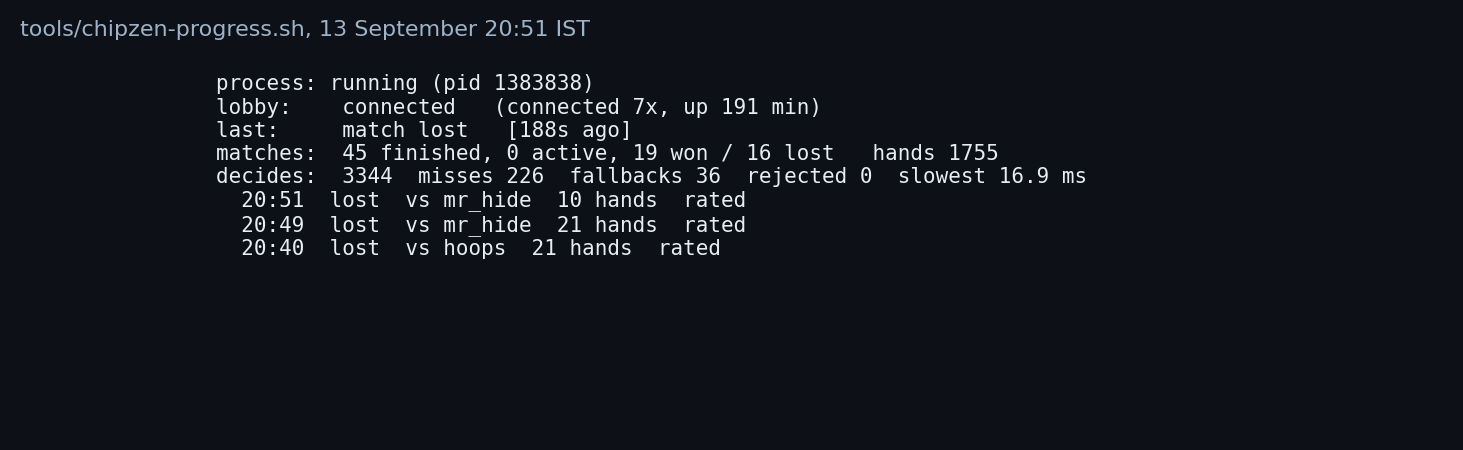
\includegraphics[width=12.2cm]{snap_progress.png}
\caption{The progress reader during the 13 September session.}
\label{fig:10}
\end{figure}

\begin{figure}[t]
\centering
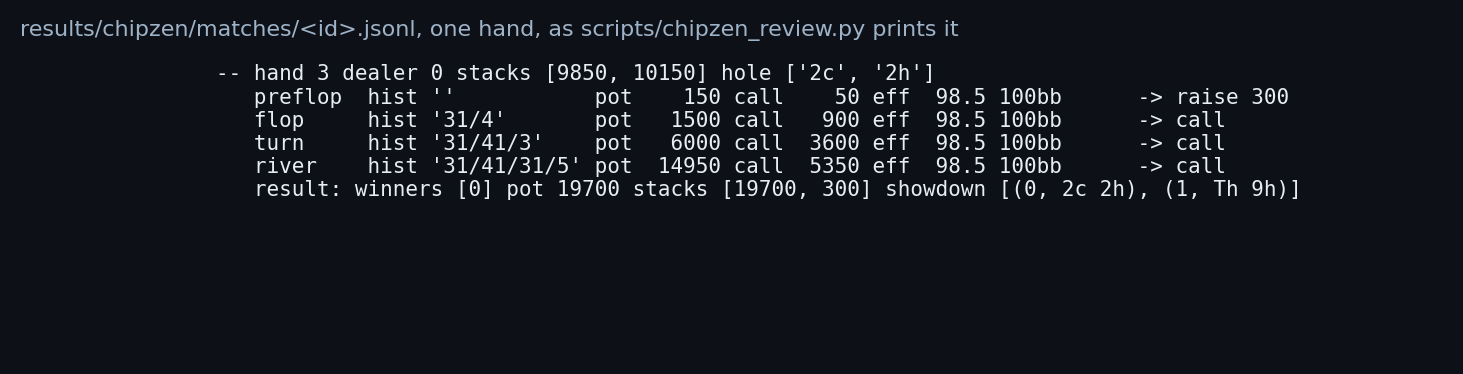
\includegraphics[width=12.2cm]{snap_decision_log.png}
\caption{One hand from the decision log: the solver called down with a pair of twos against a bluff.}
\label{fig:11}
\end{figure}

\begin{figure}[t]
\centering
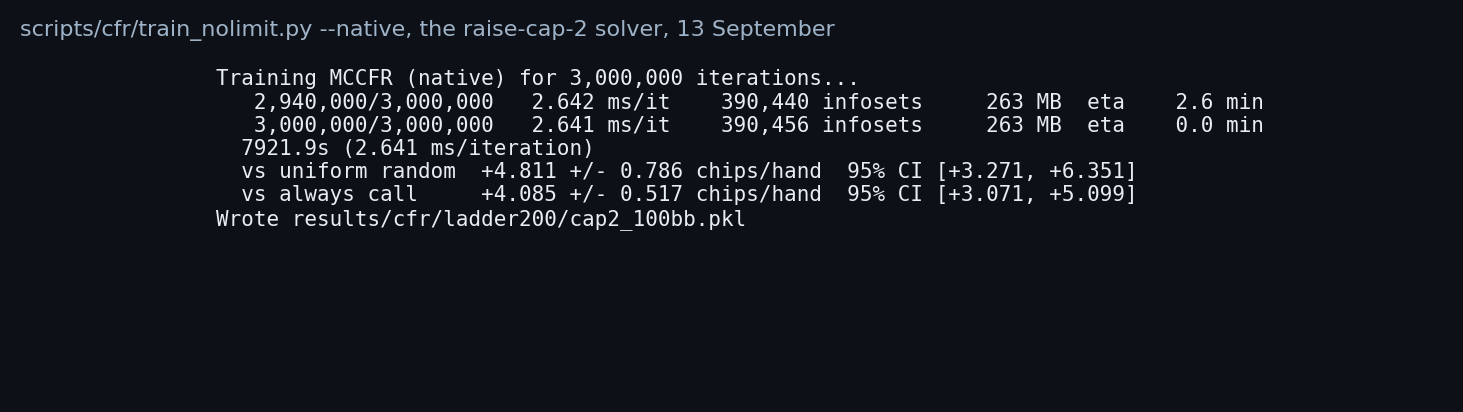
\includegraphics[width=12.2cm]{snap_training.png}
\caption{The native trainer finishing the raise-cap-2 solver.}
\label{fig:12}
\end{figure}

\section{Conclusion}
One instrument, three families, and the answer is not close: a regret-minimisation solver over a coarse abstraction beats evolutionary search by 212 BB/100 and PPO by 75, and more training does not help the learned families. The instrument mattered more than any agent: an under-trained panel had produced the opposite ranking, and only a converged panel, standard errors on every figure, and a reported miss rate made the comparison trustworthy. The abstraction findings, six buckets winning because the estimator cannot resolve more and a measured +5.9 BB/100 from sharpening it, came from the same instrument once the C++ core made experiments cheap.

Phase 2's deployment turned the instrument outward. 2,850 logged hands against other people's bots showed where a one-raise abstraction fails, deep-stacked re-raised pots, more clearly than 10,000 hands against Slumbot had, and the fixes were built and measured against the same logs. What remains is the abstraction itself: a wider betting tree measured against Slumbot with the miss rate as the gate, board-aware buckets in the main solver, and, once the logs justify one, a measured exploit rather than a guessed one.

\begin{thebibliography}{99}
\bibitem{ref1} Kuhn, H.W.: Simplified two-person poker. In: Contributions to the Theory of Games, vol. 1, pp. 97–103. Princeton University Press (1950)
\bibitem{ref2} Zinkevich, M., Johanson, M., Bowling, M., Piccione, C.: Regret minimization in games with incomplete information. In: Advances in Neural Information Processing Systems 20 (2007)
\bibitem{ref3} Lanctot, M., Waugh, K., Zinkevich, M., Bowling, M.: Monte Carlo sampling for regret minimization in extensive games. In: Advances in Neural Information Processing Systems 22 (2009)
\bibitem{ref4} Tammelin, O.: Solving large imperfect information games using CFR+. arXiv:1407.5042 (2014)
\bibitem{ref5} Brown, N., Sandholm, T.: Solving imperfect-information games via discounted regret minimization. In: Proc. AAAI (2019)
\bibitem{ref6} Johanson, M., Burch, N., Valenzano, R., Bowling, M.: Evaluating state-space abstractions in extensive-form games. In: Proc. AAMAS (2013)
\bibitem{ref7} Waugh, K., Schnizlein, D., Bowling, M., Szafron, D.: Abstraction pathologies in extensive games. In: Proc. AAMAS (2009)
\bibitem{ref8} Ganzfried, S., Sandholm, T.: Action translation in extensive-form games with large action spaces. In: Proc. IJCAI (2013)
\bibitem{ref9} Southey, F., Bowling, M., Larson, B., Piccione, C., Burch, N., Billings, D., Rayner, C.: Bayes' bluff: opponent modelling in poker. In: Proc. UAI (2005)
\bibitem{ref10} Lisý, V., Bowling, M.: Equilibrium approximation quality of current no-limit poker bots. arXiv:1612.07547 (2016)
\bibitem{ref11} Moravčík, M., Schmid, M., Burch, N., Lisý, V., Morrill, D., Bard, N., Davis, T., Waugh, K., Johanson, M., Bowling, M.: DeepStack: expert-level artificial intelligence in heads-up no-limit poker. Science 356(6337), 508–513 (2017)
\bibitem{ref12} Brown, N., Sandholm, T.: Superhuman AI for heads-up no-limit poker: Libratus beats top professionals. Science 359(6374), 418–424 (2018)
\bibitem{ref13} Brown, N., Sandholm, T.: Superhuman AI for multiplayer poker. Science 365(6456), 885–890 (2019)
\bibitem{ref14} Schulman, J., Wolski, F., Dhariwal, P., Radford, A., Klimov, O.: Proximal policy optimization algorithms. arXiv:1707.06347 (2017)
\bibitem{ref15} Heinrich, J., Silver, D.: Deep reinforcement learning from self-play in imperfect-information games. arXiv:1603.01121 (2016)
\bibitem{ref16} Brown, N., Lerer, A., Gross, S., Sandholm, T.: Deep counterfactual regret minimization. In: Proc. ICML (2019)
\bibitem{ref17} Salimans, T., Ho, J., Chen, X., Sidor, S., Sutskever, I.: Evolution strategies as a scalable alternative to reinforcement learning. arXiv:1703.03864 (2017)
\bibitem{ref18} Jackson, E.: Slumbot NL: solving large games with counterfactual regret minimization using sampling and distributed processing. In: AAAI Workshop on Computer Poker and Imperfect Information (2013)
\bibitem{ref19} Chipzen: an arena for developer-built poker bots. https://chipzen.ai, and the external-API protocol at https://github.com/chipzen-ai/chipzen-sdk (2026)
\end{thebibliography}
\end{document}
